\documentclass{beamer}
\usetheme{Boadilla}
\usepackage{ulem}
\usepackage{xspace}
\usepackage{xcolor}


\newcommand{\sse}{\textit{SSE}\xspace}
\newcommand{\ssa}{\textit{SSA}\xspace}
\newcommand{\se}{\textit{SE}\xspace}
\newcommand{\sa}{\textit{SA}\xspace}
\newcommand{\lap}{\ensuremath{{\sf Lap}}\xspace}


\beamertemplatenavigationsymbolsempty

\title[Improved Private ANOVA]{Improved Differentially Private Analysis of Variance}
\author[Marika Swanberg]{\textcolor{red}{Marika Swanberg} \and Ira Globus-Harris \and Iris Griffith \and \newline Anna Ritz \and  Andrew Bray \and Adam Groce}
\date{Reed College}

\begin{document}

\begin{frame}
\titlepage
\end{frame}

%\begin{frame}{Outline}
%  \tableofcontents
%  % You might wish to add the option [pausesections]
%\end{frame}

% Section and subsections will appear in the presentation overview
% and table of contents.
\section{Differential Privacy}

\begin{frame}{Hypothesis Tests}
Is observed data $D$ consistent with a proposed model, $H_0$ (null hypothesis)?\pause

\bigskip
% SLIDE 1
To carry out a hypothesis test: 
\pause
\begin{enumerate}
\item Compute a \textit{test statistic}, $t = T(D)$. \pause
\item Compute a $p$-value, $p = \Pr[T(D) \geq t \mid  D \leftarrow H_0]$. 
\begin{itemize}
\item Compute where $t$ falls on the reference distribution for $T$ \pause
\end{itemize}
\item Compare $p$ to a preset value $\alpha$ (usually .05). Reject $H_0$ if $p < \alpha$.
\end{enumerate}
\begin{figure}
  \includegraphics[scale=0.5]{images/pvalues}
\end{figure}
\end{frame}


% SLIDE 2
\begin{frame}{Hypothesis Tests}
A good hypothesis test: \pause
\begin{enumerate}
    \item Has a known reference distribution \pause
    \item Quickly diverges from the reference distribution if $H_0$ is false
\end{enumerate}
\pause
\begin{definition}[Power]
The \textbf{power} of a hypothesis test is the probability it rejects $H_0$.  It depends on the alternate distribution $H_A$ and $n$.
\end{definition}
\end{frame}

% SLIDE 3
\begin{frame}{Differential privacy [DMNS06]}

\begin{definition}
Two databases are \textbf{neighboring} if they differ only in the data of one individual.
\end{definition}
\pause
\begin{definition}
A query $f$ is \textbf{$\varepsilon$-differentially private} if for all neighboring databases $D, D'$ and all output sets $S$
\begin{equation*}
\Pr[f(D) \in S] \leq e^\varepsilon \Pr[f(D') \in S].
\end{equation*}
\end{definition}
\end{frame}

% SLIDE 4
\begin{frame}{Properties of differential privacy [DMNS06]}
\begin{theorem}[Post-processing]
If $f$ is $\varepsilon$-differentially private then for any (randomized) function $g$, then if $h(D) = g(f(D)$, $h$ is also $\varepsilon$-differentially private.
\end{theorem}
\pause
\begin{theorem}[Composition]
If $f$ is $\varepsilon_1$-differentially private and $g$ is $\varepsilon_2$-differentially private then if $h(D) = (g(D), f(D))$, $h$ is  $(\varepsilon_1+\varepsilon_2)$-differentially private.
\end{theorem}
\end{frame}

% SLIDE 5
\begin{frame}{Laplace mechanism}
\begin{definition}[Sensitivity]
The sensitivity $\Delta f$ of a deterministic, real-valued function $f$ on databases is the maximum over all pairs of neighboring $D, D'$ of $| f(D) - f(D') |$.
\end{definition}

\pause
\begin{theorem}[Laplace Mechanism]
Given any deterministic, real-valued function $f$ on databases, define $\widehat{f}$ as
$$\widehat{f}(D) = f(D) + Y,$$
where $Y \leftarrow \lap(\Delta f/\varepsilon)$. The Laplace mechanism is $\varepsilon$-differentially private.
\end{theorem}
\end{frame}

% SLIDE 5
\begin{frame}{Related Works}
    Not Campbell
\end{frame}

% SLIDE 6
\begin{frame}{Unique Challenges of Private Hypothesis Testing}
\begin{itemize}
    \item How to compute $p$-value? \pause
        \begin{itemize}
            \item Reference distribution is no longer closed-form \pause
            \item Solution: simulate it
        \end{itemize}
    \item Lots of tricky details \pause
        \begin{itemize}
            \item Ex: negative private estimates of standard deviation because of negative noise? \pause
            \item Solution: ask the statistician \pause
        \end{itemize}
    \item Low statistical power \pause
        \begin{itemize}
            \item Need a lot of data/impractical \pause
            \item Main point of improvement
        \end{itemize}
\end{itemize}
\end{frame}


% SLIDE 7
\begin{frame}{Particular Hypothesis Test: ANOVA}
ANOVA tests independence of two variables, one continuous and one categorical.\pause
\bigskip

$H_0=$ the within-category means are all equal \pause
\begin{equation*}
F(D) = \frac{\ssa(D)/(k-1)}{\sse(D)/(n-k)}
\end{equation*} 
\pause
\begin{equation*}
\ssa(D) = \sum_{j=1}^{k} n_j (\bar{y}_j - \bar{y})^2.
\end{equation*}
\pause
\begin{equation*}
\sse(D) = \sum_{i=1}^{n}  (y_{i}-\bar{y}_{c_i})^2.
\end{equation*}
\end{frame}

% SLIDE 8
\begin{frame}{Private ANOVA [CBRG18]}
Assume data is on the $[0,1]$ interval. \pause
\begin{theorem}
\sse has sensitivity bounded by 7.
\end{theorem}
\pause
$$\widehat{\sse}(D) = \sse(D) + \lap(7/\varepsilon) $$
\pause
\begin{theorem}
\ssa has sensitivity bounded by $9 + 5/n$.
\end{theorem}
\pause
$$\widehat{\ssa}(D) = \ssa(D) + \lap\left(\frac{9+5/n}{\varepsilon}\right) $$
\end{frame}

% SLIDE 9
\begin{frame}{Private ANOVA [CBRG18]}
$$\widehat{F}(D) = \frac{\widehat{\ssa}(D)/(k-1)}{\widehat{\sse}(D)/(n-k)}$$
\bigskip

 \pause
Problem: The reference distribution is a mess. \pause
\begin{itemize}
\item Simulate it.
\end{itemize}

 \pause
Problem: The reference distribution is no longer scale free.  \pause
\begin{itemize}
\item Luckily, $\widehat{\sse}$ is a variance estimate.  \pause
\item Empirically checked: good enough, type 1 error rate bounded by $\alpha$
\end{itemize}
\end{frame}

% SLIDE 10
\begin{frame}{Private ANOVA [CBRG18]}
  \begin{figure}
  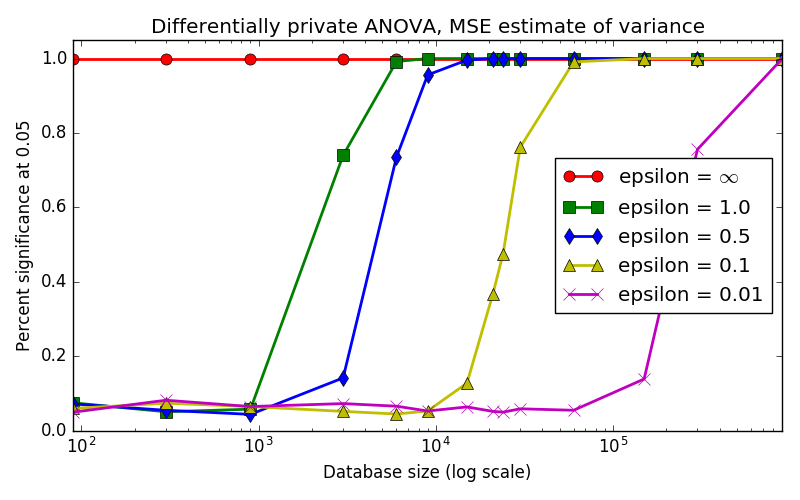
\includegraphics[scale=0.5]{images/campbellpower}
  \end{figure}
\end{frame}

% SLIDE 11
\begin{frame}{Improving ANOVA [\textcolor{red}{S}HGRGB19]}
Create a new test statistic! \pause
\begin{align*}
\ssa(D) = \sum_{j=1}^{k} n_j (\bar{y}_j - \bar{y})^2  &\Longrightarrow \textcolor{blue}{ \sa(D) = \sum_{j=1}^{k} n_j |\bar{y}_j - \bar{y}| }\\  
\sse(D) = \sum_{i=1}^{n}  (y_{i}-\bar{y}_{c_i})^2  &\Longrightarrow \textcolor{blue}{\se(D) = \sum_{i=1}^{n}  |y_{i}-\bar{y}_{c_i}| } \\  
F(D) = \frac{\ssa(D)/(k-1)}{\sse(D)/(n-k)} &\Longrightarrow  \textcolor{blue} {F_1(D) = \frac{\sa(D)/(k-1)}{\se(D)/(n-k)}}
\end{align*}
 \pause
The new $F_1$ statistic has: \pause
\begin{itemize}
\item Lower sensitivity (3 for \se, 4 for \sa) \pause
\item Much higher typical value 
\end{itemize}
\end{frame}



\begin{frame}{Improving ANOVA [\textcolor{red}{S}HGRGB19]}
Making $F_1$ private \pause
\begin{enumerate}
    \item Use Laplace mechanism as in [CBRG18] \pause
    \item Simulate reference distribution for computing $p$-value
    \begin{itemize}
        \item Problem: need standard deviation \pause
    \end{itemize}
    \item Private estimate of standard deviation:  
    \begin{itemize}
        \item Allocate some of epsilon budget? \pause Makes power worse \pause
        \item Solution: derive an unbiased estimator for $\sigma$ \pause
    \end{itemize}
\end{enumerate}
\bigskip

$$\hat{\sigma} = \sqrt{\pi/2} \cdot \frac{\widehat{SE}}{(N-k)} $$
\end{frame}

\begin{frame}{Validity of $p$-values}
    \begin{figure}
  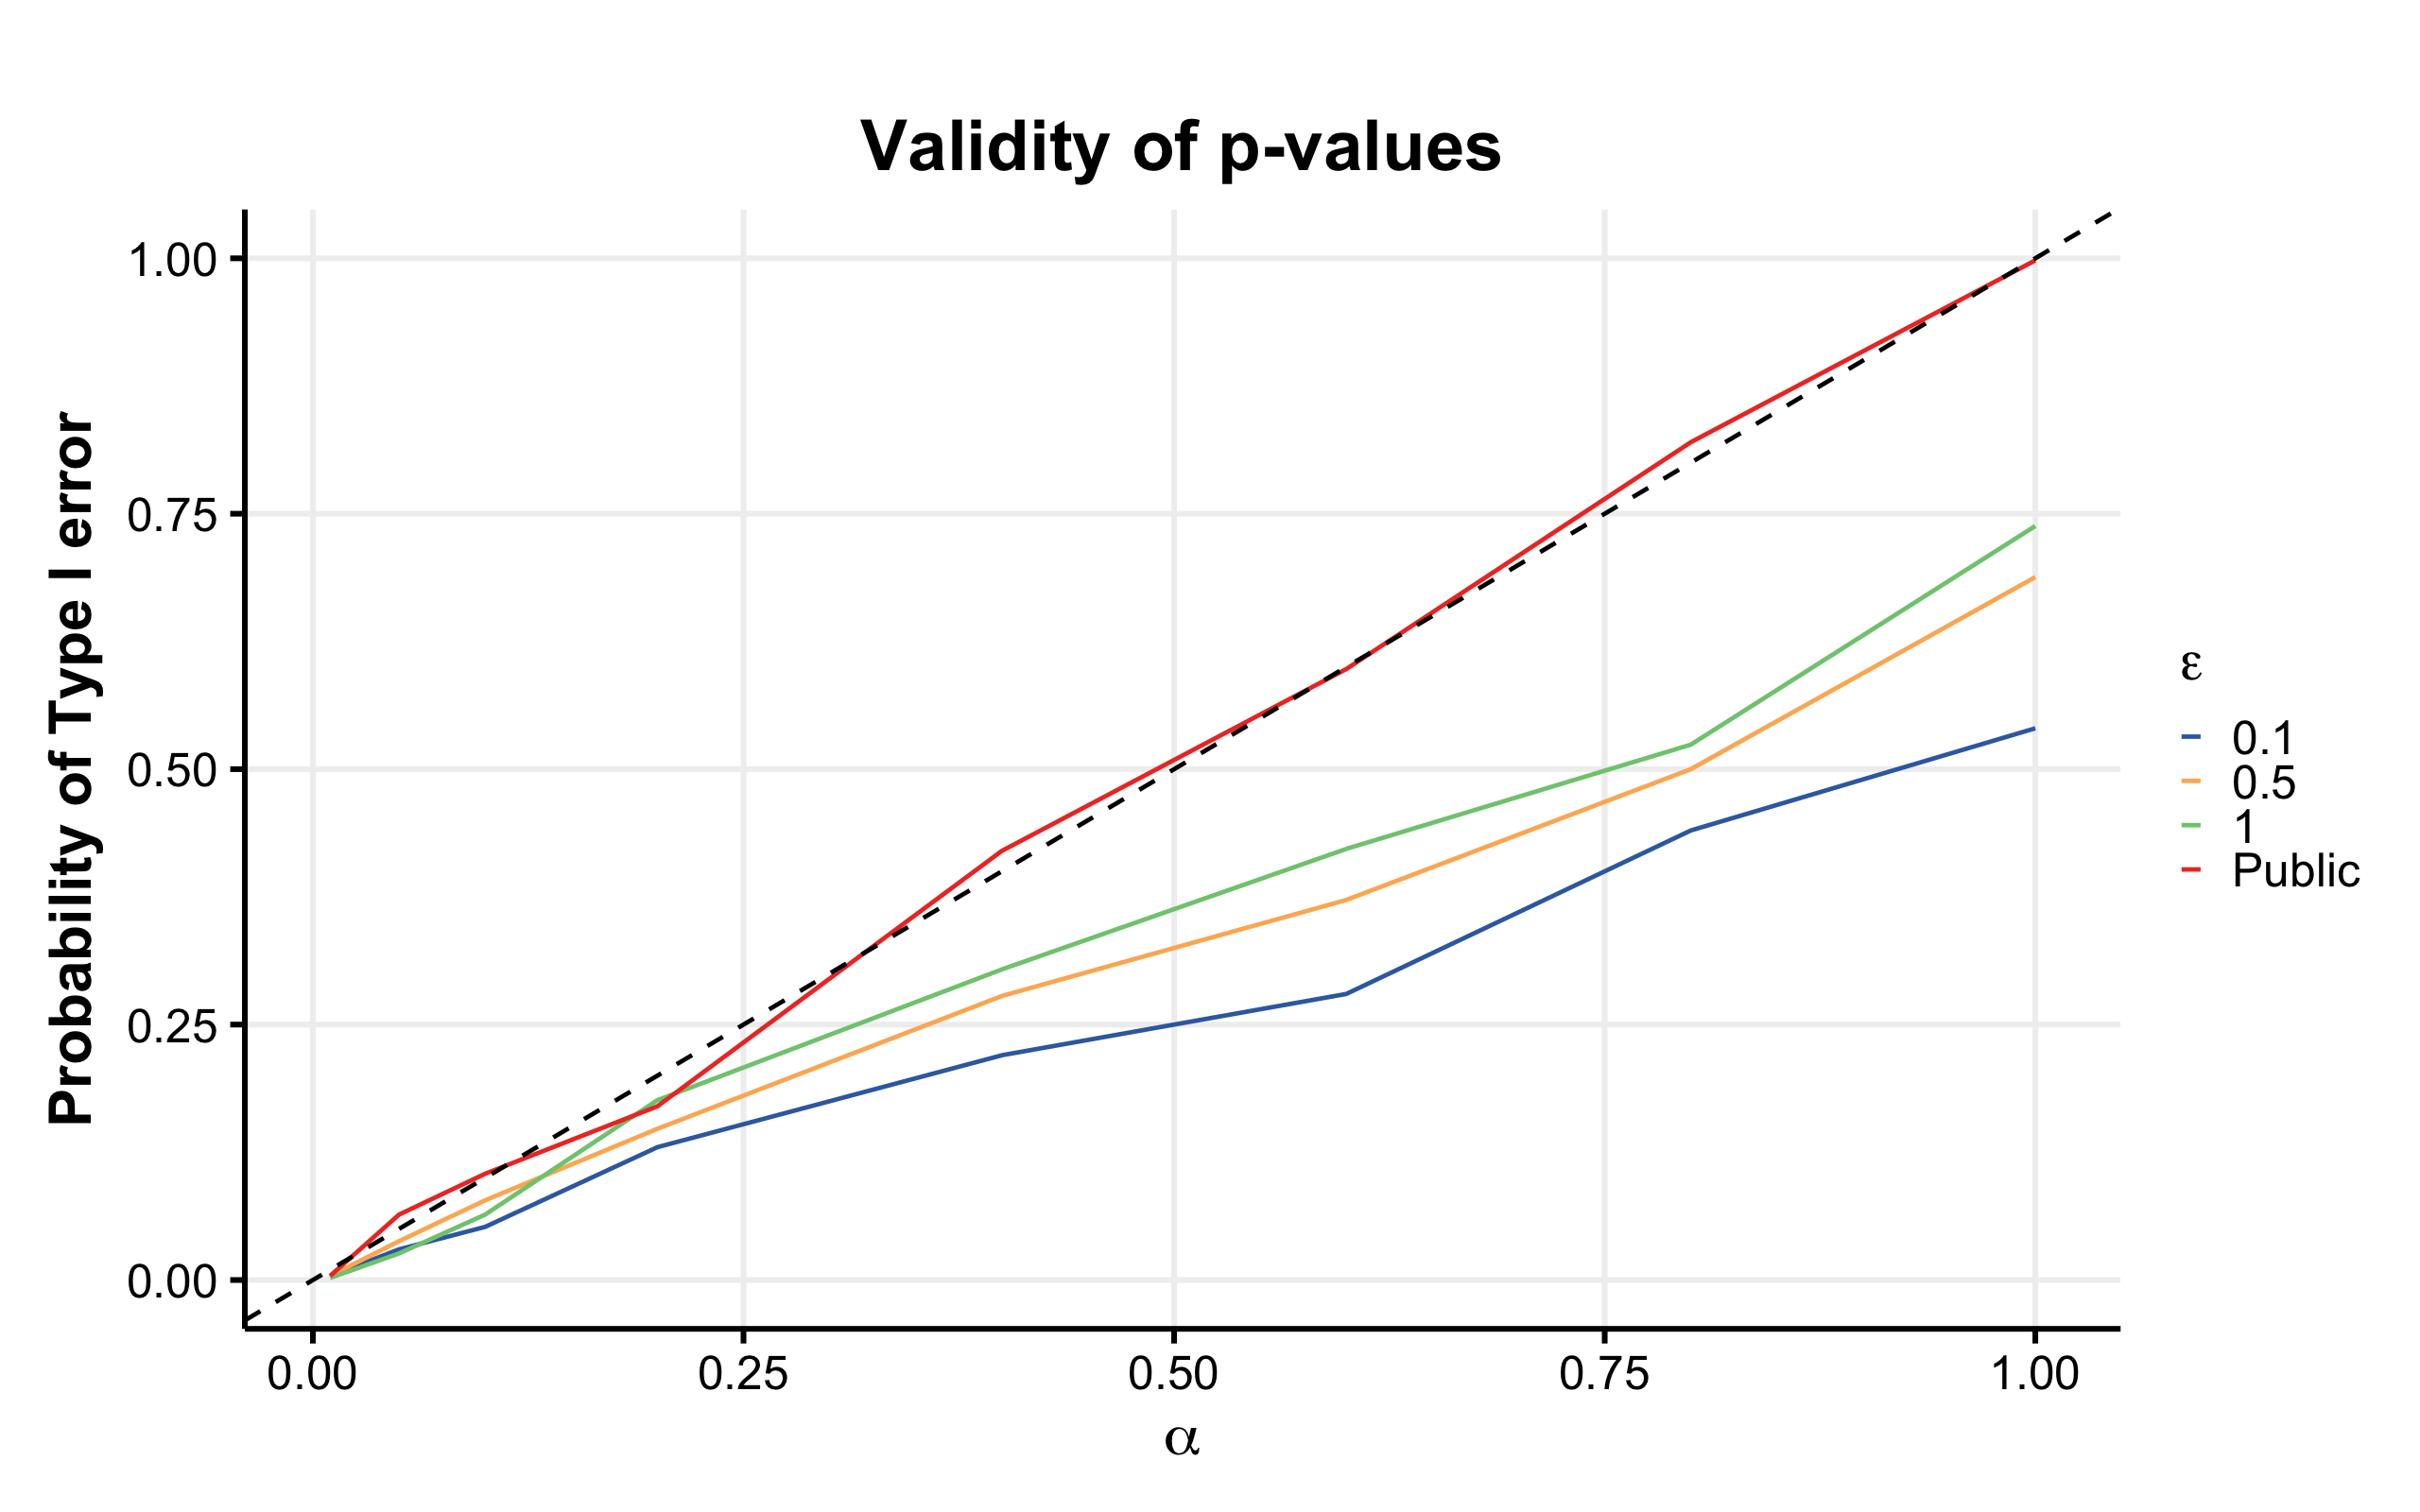
\includegraphics[scale=0.1]{images/valid-pvals}
  \end{figure}
\end{frame}


\begin{frame}{Power of $F_1$ test}
  \begin{figure}
  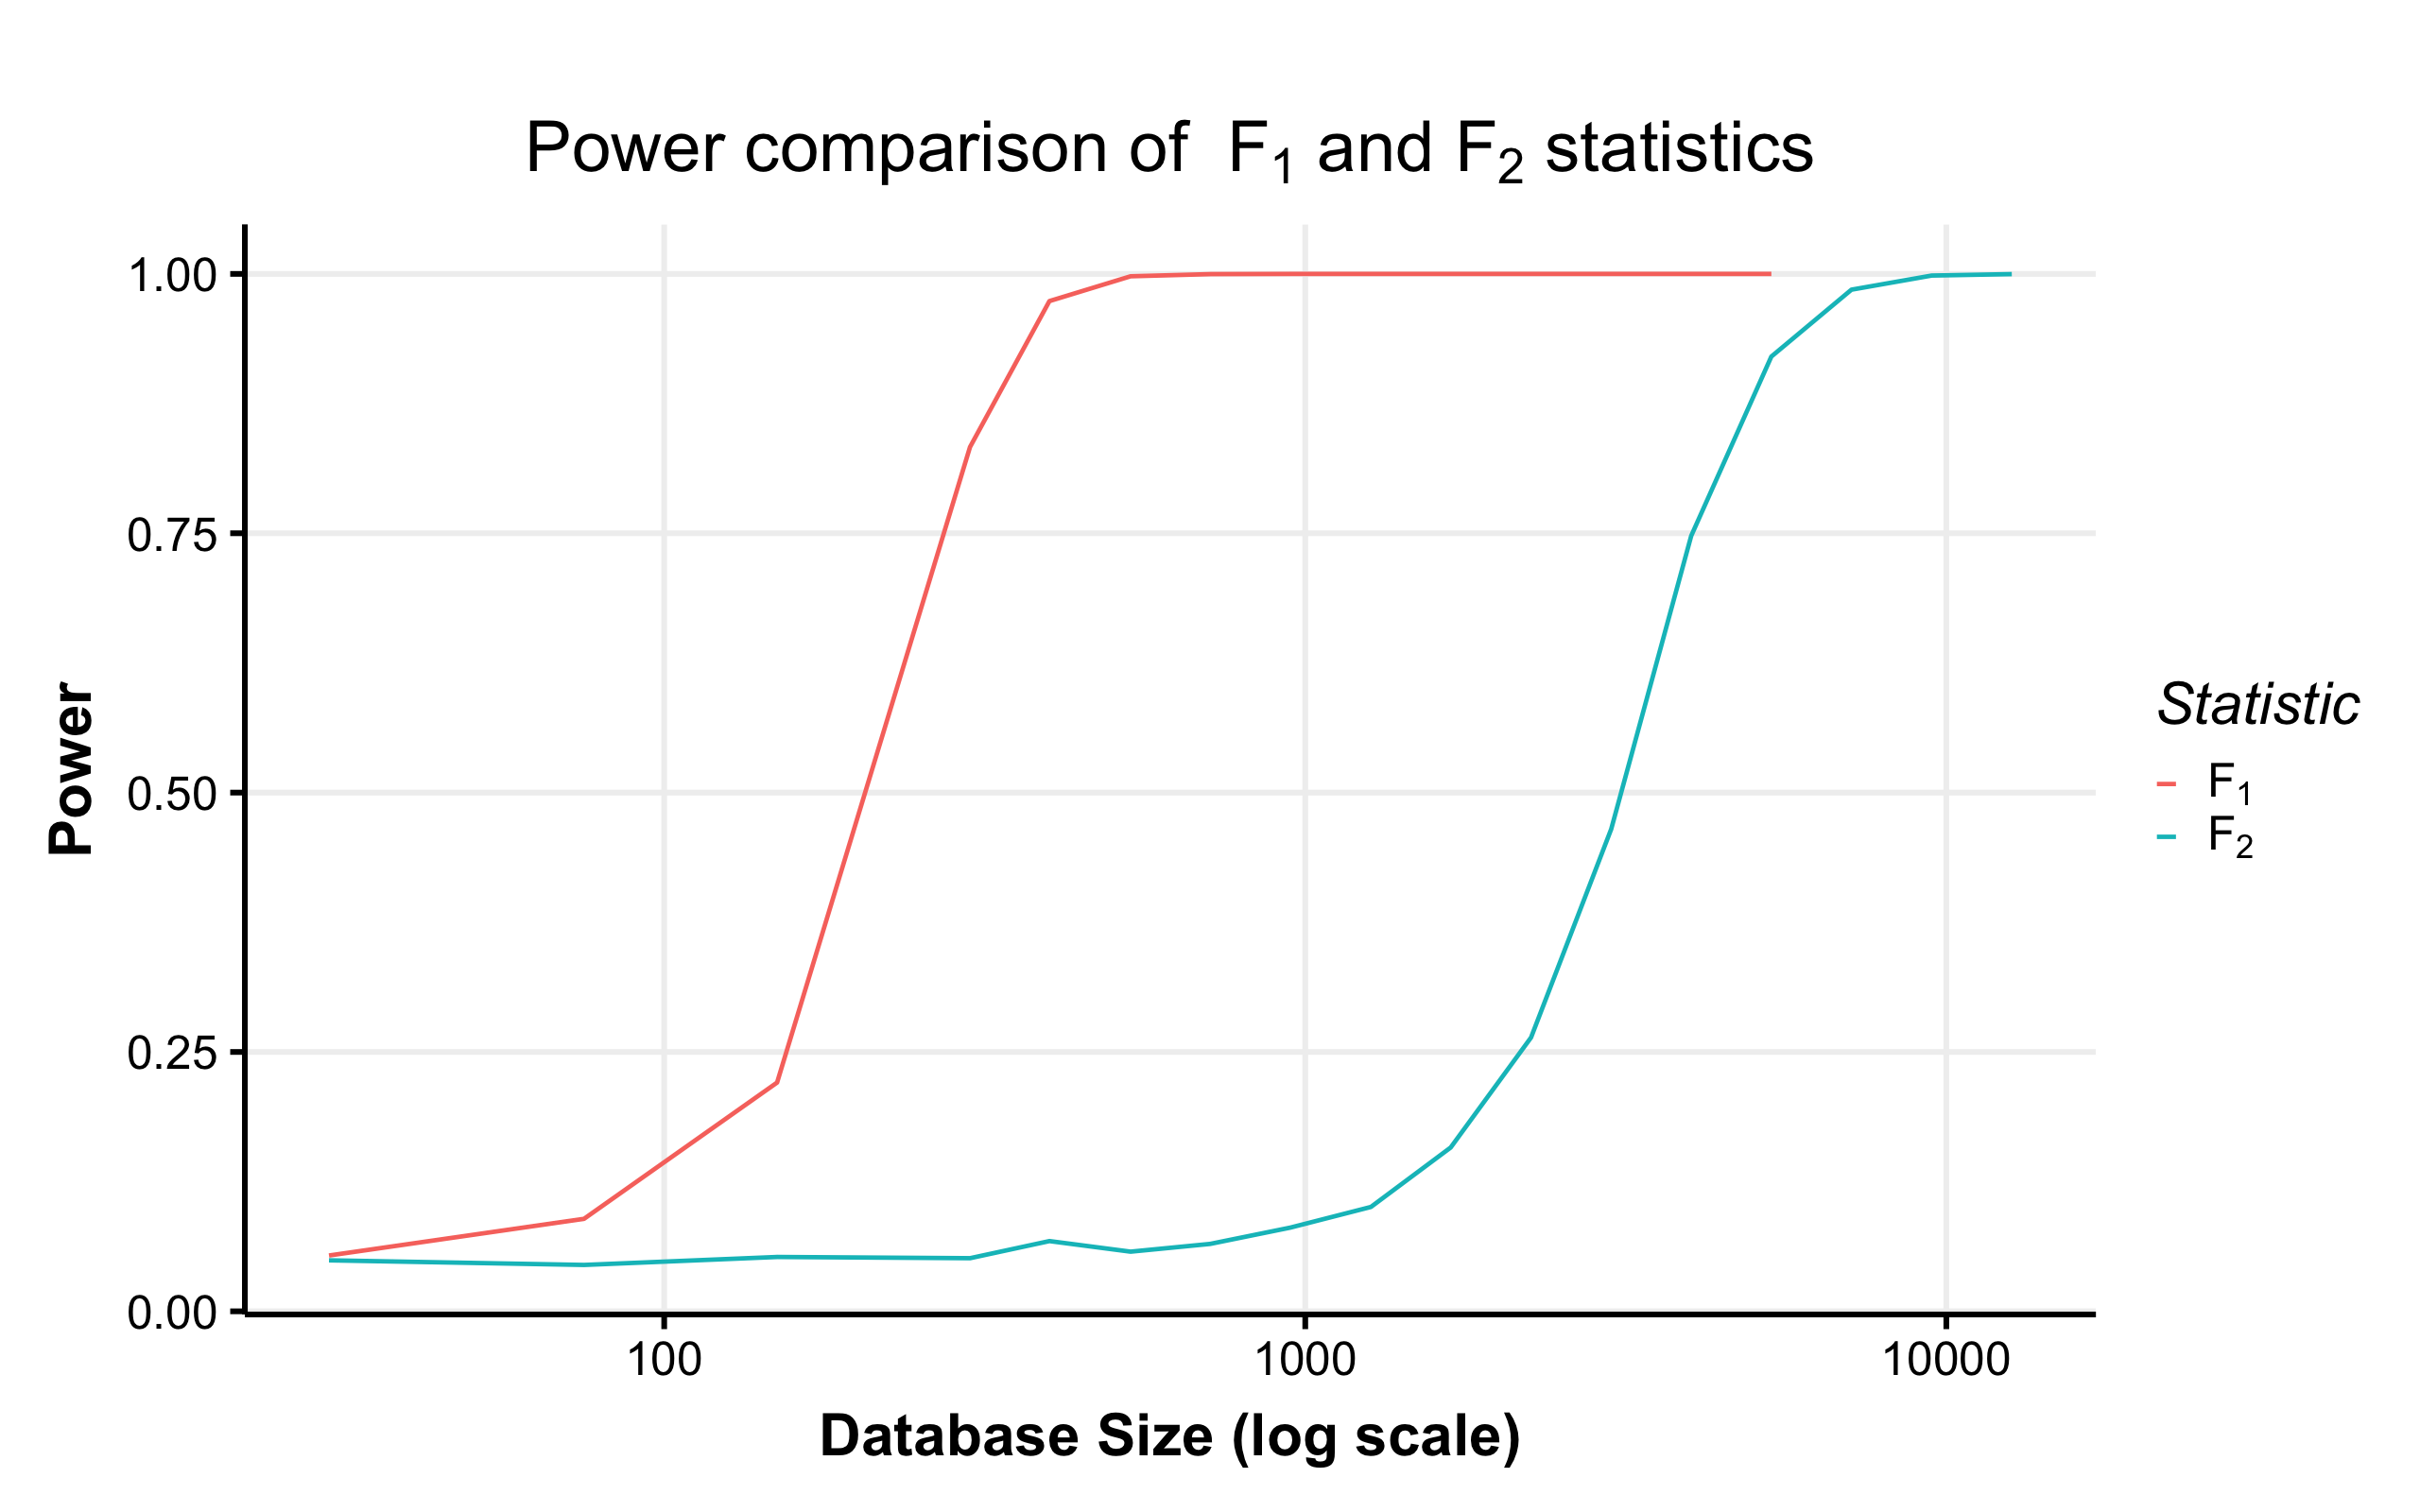
\includegraphics[scale=0.1]{images/f1-vs-f2}
  \end{figure}
  Power comparision at $\varepsilon=1$.  $F$ achieves 80\% power with 4500 observations.  $F_1$ requires 300.
\end{frame}


\begin{frame}{Further Optimization}
\end{frame}

\begin{frame}{New Developments [CKSBG19]}

Kruskal-Wallis test analogous to F-test \pause
\bigskip 

Modified KW test, similar methods as [\textcolor{red}{S}HGRGB19] \pause

\begin{figure}
  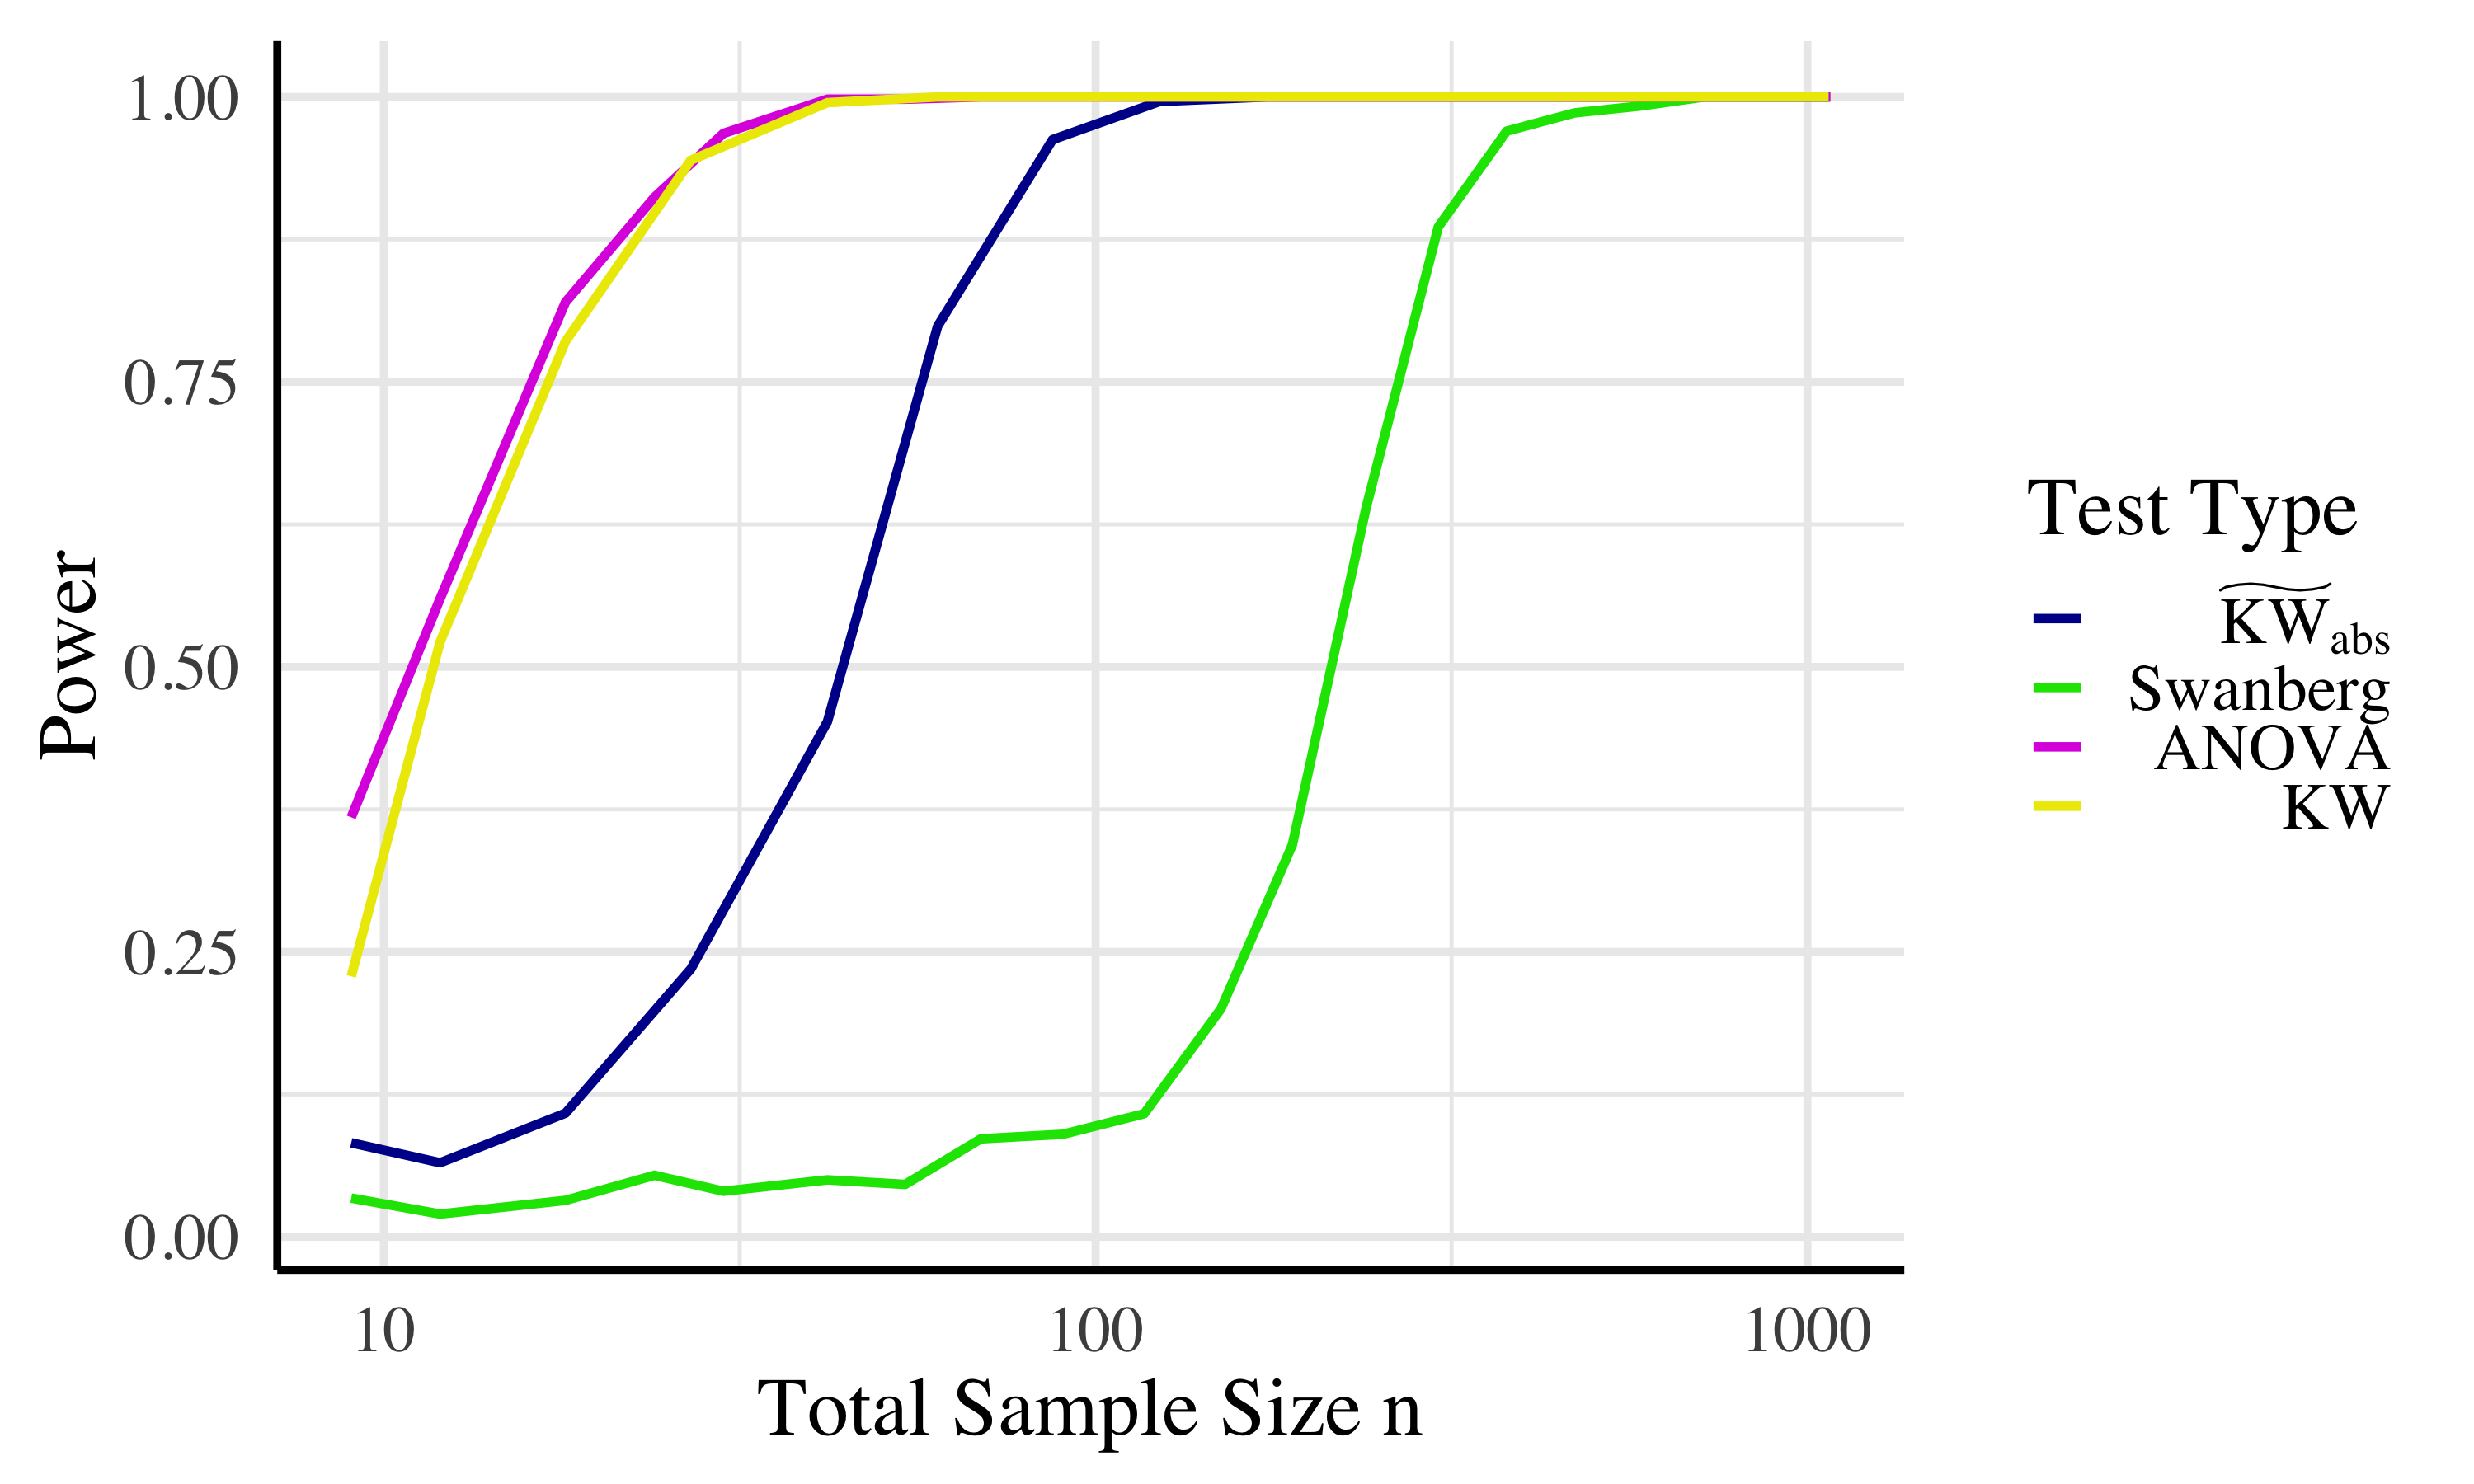
\includegraphics[scale=0.075]{images/anova_comp}
  \end{figure}
  
  For 80\% power, need only 23\% as much data as $F_1$ ([\textcolor{red}{S}HGRGB19]) \ldots \pause and about 1-2\% as much data as $F_2$ ([CBRG18])
\end{frame}

\begin{frame}{}
    \begin{center}
        \Huge Thank you
    \end{center}    
\end{frame}

% KEEP THIS SLIDE ON RELATED WORKS?
\begin{frame}{Prior work}
Other work on private hypothesis testing:\pause
\begin{itemize}
\item Asymptotic but impractical [WZ10, Smith11, CKMSU19] \pause
\item Chi-squared test (difference of discrete distributions) [VS09, FSU11, JS13, USF13, WLK15, GLRV16, RK17] \pause
\item Other tests: \pause
\begin{itemize}
\item Binomial data [AS18] (Proven optimal!) \pause
\item Difference of two means [OHK15, DNLI18] \pause
\item Survival analysis [NH17] \pause
\item Linear regression [BRMC17, Sheffet17] \pause
\end{itemize}
\end{itemize}
Earlier work is often missing: \pause
\begin{itemize}
\item Rigorous p-value computations \pause
\item Power analysis
\end{itemize}
\end{frame}



\end{document}
